\documentclass[letterpaper,twocolumn,11pt]{article}

\usepackage[utf8]{inputenc}

\usepackage{mathptmx}
\usepackage{booktabs}
\usepackage[tableposition=top]{caption}
\usepackage{float}
\usepackage{graphicx}
\usepackage{hyperref}
\usepackage{rotating}
\usepackage{titlesec}
\usepackage{tikz}

\usepackage[T1]{fontenc}

\usetikzlibrary{arrows}
\usetikzlibrary{positioning}

%\titleformat{\section}{\normalfont\scshape}{\thesection}{1em}{}

\title{Tunneling TCP Traffic over FTP}
\author{Andrew Stange \and Ryan Wails}

\begin{document}
\maketitle

\begin{abstract}
  In this report, we discuss TCP-over-FTP (ToF), a protocol tunnel we designed
  that disguises arbitrary TCP protocols as FTP. We implemented ToF in python3
  and evaluated ToF's security and performance properties. We conclude the
  report by discussing aspects of ToF's design and how techniques for protocol
  obfuscation further make obsolete the distinctions between Internet packet
  data and metadata.
\end{abstract}

\section{Introduction}

Protocol obfuscation is the practice of disguising one Internet protocol as
another, and is used as a surveillance and censorship countermeasure. For
example, a protocol obfuscation technology might pass HTTP web traffic through
an audio modem and tunnel the traffic over Skype, which would \emph{disguise}
the HTTP traffic as Skype voice traffic.

In this work, we present TCP-over-FTP (ToF), an obfuscating protocol tunnel designed
to disguise arbitrary TCP protocol messages as messages occurring in an file
transfer protocol (FTP) session. A user running ToF could freely browse the
web, for instance, but would appear to be transferring files with a fixed FTP
server. We implemented a prototype of ToF in python3, and verified that we were
able to browse the web over ToF using Firefox.

Protocol and connection endpoint obfuscation technologies have implications for
law enforcement practices. For example, using a pen register, law enforcement
officials are able to monitor the endpoints of an electronic communication
transmission without a warrant. But, obfuscation technologies hide details like
endpoint IP addresses and TCP protocols inside packet payloads (which may not
be accessible using a pen register). We discuss these implementations in more
detail in \S\ref{sec:discussion}.

This work is organized as follows. In \S\ref{sec:background}, we give
background details on the file transfer protocol and protocol obfuscation
techniques. In \S\ref{sec:system}, we present ToF's design, give details of our
prototype implementation, measure ToF's performance, and discuss aspects of
ToF's security. Finally, in \S\ref{sec:discussion}, we conclude by discussing
(1) distinctions between ToF and similar technologies, (2) difficulties in
implementing ToF, and (3) the broader implications of protocol obfuscation
technologies.

\section{Background and Related Work} \label{sec:background}

\subsection{File Transfer Protocol}

With proposals dating back to the 1970s, the File Transfer Protocol (FTP) is
one of the older network protocols still used today \cite{ftprfc}. FTP
interactions are carried out between a client and server. After
authenticating with the server, the client can issue a number of commands to
manipulate directories and files on the server, including:

\begin{itemize}
  \item \texttt{CWD}: Change the remote working directory
  \item \texttt{LIST}: List the files in the remote working directory
  \item \texttt{SEND}: Upload a file to the remote working directory
  \item \texttt{RECV}: Download a file from the server
\end{itemize}

Not unlike other legacy protocols, FTP authentication and data transfers occurs
``in the clear'', without using cryptographic technologies like encryption and
authentication to protect data. Without encryption, eavesdroppers on the
network can view the client's credentials and the contents of files transferred
between the client and the server, which may also be sensitive. Secure variants
of FTP have been developed, including SSH FTP (SFTP) and FTP with TLS (FTPS)
\cite{sftp-draft, ftpsrfc}. These variants use mature cryptographic protocols
(secure shell and transport layer security, respectively) to encrypt and
authenticate messages between the client and the host. When observing a
connection made using these secure FTP variants, a network eavesdropper can
measure packet sizes and transmission times, but cannot inspect payload
contents.

\subsection{Protocol Tunneling and Misidentification}

\emph{Protocol identification} is a common goal of network investigators and
network security appliances. Since data flows between pairs of network hosts
can be arbitrary, measurement and inference must be performed to determine
which protocols are generating the flows. Identification techniques are often
simple (for example, using TCP port numbers to infer protocols), but newer
``deep packet inspection'' techniques achieve higher identification accuracy
using more complex algorithms (for example, using machine learning
classification with the packet payloads as the features).

\emph{Protocol misidentification} (also known as \emph{protocol obfuscation})
is the practice of disguising the genuine protocol being used (sometimes called
the \emph{covert} protocol) as another ``alibi protocol'' (sometimes called the
\emph{cover} protocol).  For example, a client using a protocol
misidentification tool might be browsing the web, but network traffic generated
by the host would appear to be email traffic.

A common technique to achieve protocol misidentification is through
\emph{tunneling}. In tunneling schemes, the cover protocol is run correctly
between the hosts, but the covert protocol messages are embedded within the
cover protocol messages. Continuing the previous example, the web-over-email
misidentification tool could embed HTML messages as email attachments or even
as
uuencoded\footnote{\url{https://pubs.opengroup.org/onlinepubs/9699919799/utilities/uuencode.html}}
text in the email body.

A notable use of protocol obfuscation is by the Tor Project in the live Tor
network \cite{tor}. Obfuscated transports like ScrambleSuit and Format-Transforming
Encryption have been deployed to help users in censored networks connect to the
Tor network while disguising Tor protocol messages \cite{scramblesuit, fte}.
As of 2021, Tor Metrics reports that more than 40,000 users connect to Tor
using the obfs4 obfuscated transport, which disguises Tor protocol messages to
look like uniformly-random, unstructured bytes.

Researchers have considered many alternatives for protocol tunneling that have
not been deployed publicly.  Several works have proposed tunnels through VoIP
and video conferencing calls \cite{skypemorph, facet, freewave, deltashaper}.
Hahn et al. and Vines and Kohno explored low bandwidth channels using networked
video games as the cover channel \cite{castle, rook}. Email has been proposed
as an obfuscated transport for microblogging and web surfing \cite{mailet,
sweet}. Perhaps the most similar system to our FTP-based tunnel is
CloudTransport, which tunnels traffic over cloud storage protocols
\cite{cloudtransport}.

\section{TCP-over-FTP} \label{sec:system}

This section presents TCP-over-FTP (ToF), the tool we developed for protocol
misidentification. ToF tunnels arbitrary TCP traffic over FTP between a client
and proxy through an intermediary server. In \S\ref{subsec:design}, we present
the design of our tool. In \S\ref{subsec:impl}, we give details about our
prototype implementation of ToF. Then, in the final subsections, we evaluate
the performance and security properties of our design and implementation.

\subsection{Protocol Design} \label{subsec:design}

\begin{figure*}[t]
  \centering
  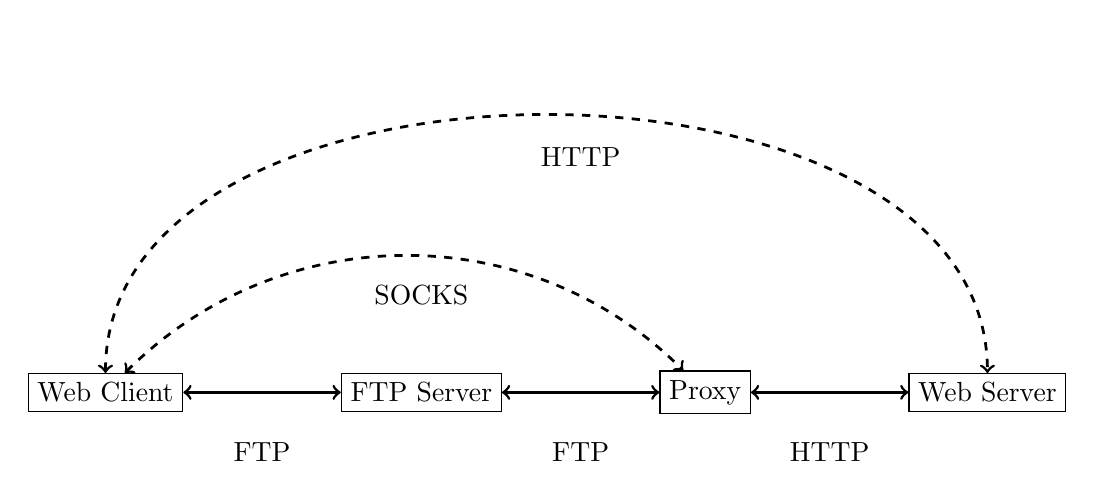
\begin{tikzpicture}

\node[draw] (a) at (0,0) {Web Client};
\node[draw, right = 2cm of a] (b) {FTP Server};
\node[draw, right = 2cm of b] (c) {Proxy};
\node[draw, right = 2cm of c] (d) {Web Server};

\node[above = 0.75cm of b] () {SOCKS};

\draw [to-to,line width=1pt](a) -- (b) node [midway, fill=white, below=0.5cm] {FTP};
\draw [to-to,line width=1pt](b) -- (c) node [midway, fill=white, below=0.5cm] (mid) {FTP};
\draw [to-to,line width=1pt](c) -- (d) node [midway, fill=white, below=0.5cm] {HTTP};
\draw [to-to,line width=1pt, dashed](a) to [out=45,in=135] (c);
\draw [to-to,line width=1pt, dashed](a) to [out=90,in=90] (d);

\node[above = 3.25cm of mid] () {HTTP};

\end{tikzpicture}

  \caption{Communication topology of a TCP-over-FTP connection carrying HTTP
  traffic. Solid edges denote direct connections between hosts. Dashed
edges denote logical (tunneled) connections between hosts.}
  \label{fig:topology}
\end{figure*}

In ToF, a \emph{client} and \emph{proxy} communicate via FTP through an
intermediary server. Both the client and proxy run custom FTP client software,
and the server runs an unmodified instance of the FTP server protocol.
First,
the client and proxy negotiate a session. After session negotiation phase, the
client and proxy enter a data transmission phase where the client and proxy
exchange SOCKS messages carrying TCP traffic encoded as FTP files
(discussed further below). The communication topology for an instance of the
ToF protocol carrying HTTP traffic is shown in Figure~\ref{fig:topology}.

\subsubsection{Session Negotiation Phase} \label{subsubsec:session}

During session negotiation, the client and proxy negotiate a symmetric key $k$
and a file naming convention for the session. The file naming convention is
used to associate files on the FTP server with client-server sessions and to
order the messages.  For example, a client and server can agree that filenames
for the stream follow the pattern \texttt{stream\_$i$}, where, e.g., file
\texttt{stream\_3} contains the 3rd message of the session.

\begin{figure*}[t]
  \centering
  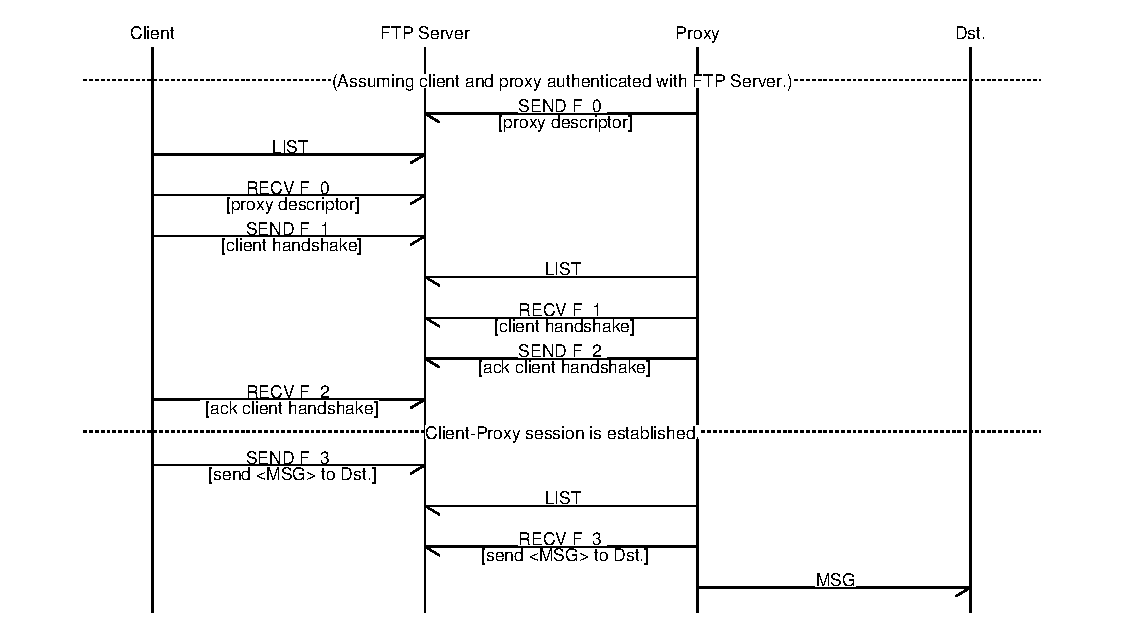
\includegraphics[width=\textwidth]{tof_seq}
  \caption{Message sequence diagram showing client-proxy session negotiation
    and message proxying. Messaged labeled F\_\{1,2,3,4\} denote
  file transmissions with sequential filenames.}
  \label{fig:msgseq}
\end{figure*}

Figure~\ref{fig:msgseq} shows the session negotiation process in more detail.
The steps to the session negotiation process are as follows:
\begin{enumerate}
  \item The proxy sends a proxy descriptor file that containing the public
    key and filename convention of the proxy. The descriptor filename uses a
    format known to the client.
  \item The client receives the proxy descriptor and learns the public key and
    filename convention of the proxy.
  \item Using the proxy's filename convention hereafter, the client sends a
    handshake file containing a randomly-chosen session key $k$ and the
    client's identify encrypted under the proxy's public key.
  \item The proxy receives the handshake. If the proxy can successfully decrypt
    the client's handshake message using its private key,
    it saves the session key $k$ and sends a final acknowledgement message.
  \item The client receives the acknowledgement message and learns that the
    proxy is ready for data transmission.
\end{enumerate}

Between file transmissions, the client and proxy periodically poll the FTP
server using the \texttt{LIST} command to check for new files.

\subsubsection{Data Transmission Phase} \label{subsubsec:transmission}

After the client and proxy have negotiated a session key and know to listen for
messages from each other, they proceed to the data transmission phase. During
data transmission, the client and proxy exchange binary files containing
messages generated from a SOCKS-client and SOCKS-proxy instance running on the
ToF client and ToF proxy, respectively. SOCKS is a widely-used proxy protocol
that can be used to forward arbitrary TCP data from a user-facing application
\cite{socksrfc}.  For example, most modern web browsers, without any
modifications, can be configured to forward their traffic through a SOCKS
proxy. We chose to have ToF use SOCKS so that we could test ToF with legitimate,
SOCKS-compatible applications like web browsers.

All SOCKS messages that are sent and received to and from the FTP server are
encrypted under the session key $k$. An authenticated encryption scheme is used
between the client and proxy which provides message authentication and
confidentiality---in particular, the encryption scheme prevents the FTP server
from reading or modifying SOCKS messages.

\subsection{Prototype Implementation} \label{subsec:impl}

We implemented ToF in approximately 700 lines of python3 code. We used python's
standard \texttt{ftplib} package for the FTP client. The prototype supports
legacy FTP and FTPS (FTP over TLS). We use a modified version of the
open-source \texttt{PySecretSOCKS}
package\footnote{https://github.com/Drewsif/PySecretSOCKS} to implement the
SOCKS client and proxy. \texttt{libsodium} with python bindings is used to
implement ToF's public-key and private-key cryptography functionalities.

We tested ToF on Ubuntu Linux v20.04 and python v3.8.5. The source code for ToF
is available and attached along with this report.

\subsection{Performance Evaluation} \label{subsec:eval}

To measure system performance, we ran a client, server, and proxy, and measured
the performance of a network download.

We deployed a virtual private server to test performance in a realistic network
model. We rented the VPS on Digital Ocean and provisioned it with a 1 Gbps
symmetric network link and imaged it with Ubuntu Linux v20.04 and the vsftp FTP
server v3.0.3. The machine was physically hosted in New York City and was
connected in AS14061 (Digital Ocean). In this performance evaluation, the proxy
was co-located on this VPS, which likely makes our performance measurements
optimistic (because we are shortening a network hop between hosts).

We ran the client running in residential AS7922 (Comcast Cable) with a 300~Mbps
download speed and 10~Mbps upload speed network link. The client was directed
to download a 1~MiB file hosted at \url{speedtest.tele2.net} over HTTP with the
\texttt{curl} command line tool. The transfer took 133~seconds to complete,
yielding a goodput of 63~kbps. In comparison, the client could perform the
download in approximately 1~s (8 Mbps)---for this transfer, the slowdown due to
ToF was approximately $133\times$. During the transfer, the client transmitted
1.7~MB and received 6.5 MB to transfer the 1~MiB file.

Despite these large overheads, ToF might still be useful in some settings. We
were able to connect Firefox to ToF, and were able to browse the web over FTP.
Page load times varied significantly by host, but usually took a few minutes
to visit simple websites. A video of ToF being used with Firefox can be found
here: \url{https://www.youtube.com/watch?v=90Bhn_oM1ZM}.

\subsection{Security Discussion} \label{subsec:security}

\subsubsection{Confusing IDS Tools}

The primary goal of ToF is to disguise arbitrary TCP protocols as FTP. Indeed,
we verified that HTTP connections made through ToF are identified as FTP by
network analysis tools. Wireshark v3.4.5 and Zeek v4.1.0 both label flows
created by ToF as FTP (the flows are \emph{not} labeled as HTTP, even though
the flows were carrying HTTP traffic).  (Zeek is the most recent version of
Bro, a popular open-source intrusion detection system proposed in 1998 by Vern
Paxson \cite{bro}.) This result is not surprising, because these network
analysis tools are not aware of ToF and ToF does faithfully execute the FTP
protocol to transmit data.

However, strong security systems should be designed with Kerckhoffs's principle
in mind---the system should remain secure \emph{even when} the adversary or
observer knows of its existence and construction. ToF likely does not provide
strong security under this assumption: ToF traffic has characteristics that
look highly irregular when compared to ordinary FTP traffic. For instance, ToF
regularly issues the \texttt{LIST} command to watch for changes in the working
directory (to maintain data transfer performance, the \texttt{LIST} command is
issued every few milliseconds). Looking for the prevalence of these short
messages, even if secure FTP is used, would probably work to identify ToF
sessions.

ToF is best suited as a tool to confuse dragnet, unsophisticated attempts at
surveillance. Strong, targeting adversaries could probably learn a lot using
the cover protocol's packet sizes, directions, and times.

\subsubsection{Hiding Connection Endpoints}

ToF offers a bonus security property: connection endpoints are also obfuscated
by our network topology. A local eavesdropper monitoring a ToF client's
connections cannot see the actual destination being connected to by the client.
Instead, the eavesdropper sees the ``alibi'' connection to the FTP server.
Even if the eavesdropper has control of the FTP server, he or she can see the
network identity of the client and proxy \emph{but not} the destination (the
end-to-end encryption used between the client and proxy prevent the server from
looking at SOCKS protocol messages to learn this information).

An eavesdropper would need to establish multiple observation points in the
wider network to directly link the client to the destination, significantly
raising the difficulty of surveillance efforts.

\section{Discussion} \label{sec:discussion}

To conclude, we will briefly discuss three topics related to ToF: (1)
distinctions between ToF and similar technologies, (2) the difficulties of
traffic shaping, and (3) the broader implications of protocol obfuscation.

\subsection{Distinctions between ToF, VPNs, and Tor}

VPNs and Tor both offer similar protections to ToF---they both obfuscate
connection endpoints, and offer connection tunneling and network packet
proxying. A key difference between these approaches and ToF is that VPNs and
Tor do not try to disguise their messages, so an eavesdropper can easily learn
these protocols are being used. Moreover, these protocols are used only for
traffic tunneling, which reveals some information about the client's behavior.
In contrast, ToF offers an additional protection: it is difficult for an
eavesdropper to determine if a client is legitimately making file transfers
over FTP, or if the client is using ToF to tunnel traffic. This protection
further obscures a client's behavior, frustrating surveillance efforts.

\subsection{Difficulties of Traffic Shaping}

As discussed in \S\ref{subsec:security}, characteristics of ToF FTP sessions
appear out-of-the-ordinary (for example, the rate of commands issued from the
client to the FTP server is extremely high). An improved design for ToF might
include \emph{traffic shaping}, which limits cover protocol actions to more
closely model genuine user behavior. However, two obstacles exist that future
work could address:
\begin{enumerate}
  \item To our knowledge, there is no ground-truth dataset for FTP behaviors.
    Without such a dataset, it is difficult to determine a set of realistic
    behaviors to emulate in the ToF protocol.
  \item ToF already comes with a substantial performance overhead. Adding
    additional message delays to more closely model human behavior could be
    challenging without further reducing the goodput of the tunneled protocol.
\end{enumerate}

\subsection{Broader Implications of Protocol Obfuscation} \label{subsec:broad}

We believe techniques like protocol obfuscation further diminish the
distinction between communication content and metadata. When applying a pen
register to Internet communication, a judgement must be made on what
information concerns ``the substance, purport, or meaning of that
communication'' \cite{us-code18-2510}---this information is defined as content
and not available to law enforcement officials using a pen register.

A reasonable stance could be taken that TCP payload data is considered
content and TCP/IP header data (in particular, the
source and destination IP addresses and port numbers) is considered metadata.
Then, it could further be assumed that the application protocol or service used
would also be considered metadata, because the Internet service in use can
often be inferred by destination port (the Internet Assigned Numbers Authority
maintains a registry of services assigned to TCP port
numbers\footnote{\url{https://www.iana.org/assignments/service-names-port-numbers/service-names-port-numbers.xhtml}}).

However, protocol obfuscation techniques like ToF meddle with this assumption.
To observe a ToF client's tunneled connection's true destination and
port/service, an investigator \emph{must} inspect the TCP payload as the outer
TCP header obscures this information.

A different stance would be to assume that IP and TCP header information are
defined as content and not metadata. However, this stance is not logically
consistent with phone wiretap legislation, which considers dialing information
(for example, the phone numbers used in the call) to be metadata and not
content.

A third possible stance is that IP header data is considered metadata, but TCP
header data is considered content. But, proxy technologies (e.g., VPNs or Tor)
hide IP addresses within packet payloads, and so this stance runs into problems
similar to the first.

Due to these inconsistencies, we recommend that new surveillance legislation be
crafted and applied to Internet traffic, instead of trying to apply law that
was originally designed for analog, voice telecommunication systems. Due to
technologies like application proxies and protocol misidentification, we
recommend that surveillance legislation should not try to distinguish content
from metadata.

\global\csname @topnum\endcsname=0

%\newpage
\bibliographystyle{plain}
\bibliography{refs}

\end{document}

